% !TeX program = lualatex
% !TeX encoding = utf8
% !TeX spellcheck = uk_UA
% !TeX root = ../EMConspect.tex

%=========================================================
\chapter{Електричне поле у провідниках}\label{\currfilebase}
\graphicspath{{\currfilebase/Pictures}}
%=========================================================
\epigraph{\Alexander  Метал --- це океан електронів, де вплив електричного поля є кермом, що задає їх рух.
}{Переосмислення ідей сучасної фізики.}


%% --------------------------------------------------------
\section{Структура провідників}
%% --------------------------------------------------------



Провідниками називають речовини, в структурі яких є вільні заряди (електрони в металах,
наприклад), які можуть переміщуватися під дією як завгодно слабких полів (рис.~\ref{tikz:metall_structure}).
\begin{wrapstuff}[o, top=0, type=figure, width=0.3\linewidth, belowsep=1em, abovesep=1em]
    \centering
	\tikzstyle{charge+}=[ball color=red!50, text=white]
	\tikzstyle{charge-}=[ball color=blue!50, text=white]
	\tikzstyle{metal}=[top color=black!15,bottom color=black!25,middle color=black!5,shading
	angle=10]

	% CONDUCTION MODEL
	\def\R{0.21} % ion radius
	\def\a{0.90} % scale
	\def\Rx{0.2*\a*\Ny}
	\def\Ry{0.5*\a*\Ny}
	\def\Nx{6} % number of ions columns
	\def\Ny{3} % number of ions rows
	\def\L{\a*(\Nx-1)} % length
	\NewDocumentCommand{\electron}{ m m m}{
		\node[charge-,draw=black,circle,fill,inner sep=0.8,scale=0.5,line width=0.3] (e) at
		({#1*\a},{#2*\a}) {$-$};
		\draw[->,green!60!black] (e) --++ (#3*0.7*\a);
	}
	\begin{center}
		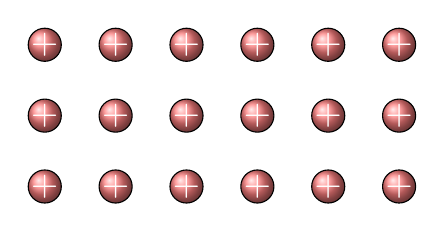
\begin{tikzpicture}[>=latex]

			% \fill[metal] (0,{-\Ry}) arc (270:90:{\Rx} and {\Ry}) --++ ({\L},0) arc (90:-90:{\Rx} and {\Ry});
			%  \draw[black!80] (0,{-\Ry}) arc (270:90:{\Rx} and {\Ry});
			%  \draw[black!80,dashed] ({\L},{-\Ry}) arc (270:90:{\Rx} and {\Ry});
			%
			% IONS
			\foreach \j [evaluate={\y=\a*(\j-\Ny/2-0.5);}] in {1,...,\Ny}{
					\foreach \i in {1,...,\Nx}{ %[evaluate={\x=\j*\a;}]
							\draw[charge+] ({(\i-1)*\a},\y) circle (\R) node[scale=1.4*\a,inner
									sep=1] {$+$};
						}
				}

			%%%%%%%%%%%%%%%%%%%%%%%%%%%%%%%%% 0
			\electron{-0.25}{ 0.55}{ -99:0.6}
			%%%%%%%%%%%%%%%%%%%%%%%%%%%%%%%%% 1
			\electron{ 0.10}{-0.55}{ 210:0.7}
			\electron{ 0.40}{ 0.35}{ 120:0.5}
			\electron{ 0.55}{ 1.30}{  10:0.6}
			%%%%%%%%%%%%%%%%%%%%%%%%%%%%%%%%% 2
			\electron{ 0.65}{-1.30}{-160:0.6}
			\electron{ 1.30}{-0.40}{  30:0.6}
			\electron{ 1.15}{ 0.40}{ 210:0.6}
			%%%%%%%%%%%%%%%%%%%%%%%%%%%%%%%%% 3
			\electron{ 2.35}{-0.70}{ -40:0.6}
			\electron{ 2.05}{ 0.55}{ -40:0.6}
			\electron{ 2.30}{ 1.30}{ -75:0.7}
			%%%%%%%%%%%%%%%%%%%%%%%%%%%%%%%%% 4
			\electron{ 3.30}{-1.30}{  20:0.5}
			\electron{ 3.40}{ 1.10}{-110:0.6}
			%%%%%%%%%%%%%%%%%%%%%%%%%%%%%%%%% 5
			\electron{ 3.38}{-0.45}{ -40:0.6}
			\electron{ 3.90}{ 0.40}{ 175:0.7}
			\electron{ 4.35}{ 1.30}{ -20:0.6}
			%%%%%%%%%%%%%%%%%%%%%%%%%%%%%%%%% 6
			\electron{ 4.45}{-0.95}{ -80:0.6}
			\electron{ 5.25}{-0.40}{  45:0.5}
			\electron{ 4.60}{-0.05}{-110:0.6}
			\electron{ 5.30}{ 0.60}{-150:0.6}
			%%%%%%%%%%%%%%%%%%%%%%%%%%%%%%%%%

			%  \draw[black!80] (0,{-\Ry}) arc (-90:90:{\Rx} and {\Ry}) --++ ({\L},0) arc (90:-90:{\Rx} and
			%  {\Ry}) -- cycle;
		\end{tikzpicture}
	\end{center}
    \caption{Структура металу\label{tikz:metall_structure}}
\end{wrapstuff}


Електронні оболонки атомів, що складають кристалічну решітку металів, сильно
перекриваються, внаслідок чого не можна вказати, біля якого іона локалізовано той чи інший
\emphx{електрон валентної оболонки}, --- вони легко перетікають від одного іона до іншого,
і, в цьому разі, кажуть, що \emphx{електрони колективізовані}. Іони --- це ядра й
електрони внутрішніх оболонок, які сильно локалізовані. Електрони, які делокалізовані,
вільно переміщаються по кристалу. Саме вільні електрони відповідають за багато фізичних і,
особливо, транспортних властивостей металів.


%% --------------------------------------------------------
\subsection*{Досліди Толмена та Стюарта}
%% --------------------------------------------------------


У 1916 р. американський фізик Р. Толмен (1881-1948) і шот\-ландсь\-кий фізик Т. Стюарт виконали
кількісні виміри, які неспростовно довели, що струм у металевих провідниках зумовлений рухом
вільних електронів.


%---------------------------------------------------------
\begin{SCfigure}[][h!]%[10]{O}{0.3\linewidth}
    \centering
    
\includegraphics[width=0.35\linewidth]{exptommstuart}
    \caption{Принципова ідея дослідної установки Толмена і Стюарта}
    \label{}
\end{SCfigure}
%---------------------------------------------------------
У цих дослідах котушку з великим числом витків тонкого дроту підключали до
гальванометра і приводили в швидке обертання навколо своєї осі. Під час різкого
гальмування котушки в колі виникав короткочасний струм, зумовлений інерцією носіїв
заряду. За напрямком відхилення стрілки гальванометра було встановлено, що
\emphx{електричний струм створюють негативно заряджені частинки}. При цьому
експериментально був отриманий питомий заряд носіїв $q/m$, близький до питомого
заряду електрона, отриманого з інших дослідів. Так було експериментально доведено,
що носіями вільних зарядів у металах є електрони.


%\href{https://www.youtube.com/watch?v=nVwquffMk44}{\color{blue}Відеодемотнстрація дослідів}

%% --------------------------------------------------------
\section{Провідник у полі}
%% --------------------------------------------------------




Якщо провідник потрапляє в поле, електрони в ньому починають рухатися проти поля.
На одній частині поверхні провідника виступає негативний заряд --- ця поверхня стає
збагаченою електронами. На протилежній частині поверхні
електронів виявляється дещо менше, ніж потрібно для нейтралізації позитивного
іонного заряду кристалічної решітки, і ця частина поверхні виявляється зарядженою
позитивно. Позитивна і негативна частини поверхні створюють своє власне поле, за
напрямком протилежне зовнішньому. Обидва поля --- зовнішнє $\Efield_\text{ex}$ і
поле власних     поверхневих зарядів провідника ($\Efield_\text{in}$) точно
компенсують одне одного в усіх точках усередині і на поверхні.

Якби в якій-небудь ділянці провідника поля $\Efield_\text{ex}$ і $\Efield_\text{in}$
не компенсували одне одного, то в цій ділянці на електрони діяла б сила і йшов би
струм. Відсутність струму означає повну компенсацію полів.


%=========================================================
\begin{figure}[h!]\centering
%---------------------------------------------------------
\begin{subfigure}[t]{0.45\linewidth}\centering
	\begin{tikzpicture}[>=latex]
		\clip (-3, -2.6) rectangle (3,2.6);
		\pgfmathsetseed{9}
		\draw[ball color=gray!5, name path=metall, smooth] plot [smooth cycle,
				samples=8,domain={1:10}]
		(\x*360/10+5*rnd:0.5cm+1cm*rnd);


		\foreach[] \y in {-3,...,3} {
				\draw[->, red] (-3, 0.6*\y) -- ++(6, 0);
			}

		\foreach[count=\c] \y in {-3,...,4} {
				\path[name path global=Q\c] (-2, 0.25*\y) -- ++(4, 0);
			}

		\foreach \c in {1,...,7} {
				\path[name intersections={of=metall and Q\c}]  (intersection-1)
				node[anchor=center, right,
					text=blue, font=\tiny] (A\c) {$-$}
				(intersection-2)  node  [anchor=center, left,
					text=red, 							font=\tiny] (B\c) {$+$} ;
				\draw[->, red, densely dashed] (B\c) -- (A\c);
			};
		%			\path (-3,2.23) node (x) {} -- ++(6,0);
	\end{tikzpicture}
\caption{Перерозподіл зарядів до встановлення рівноваги}
\label{}
\end{subfigure}
%---------------------------------------------------------
\begin{subfigure}[t]{0.45\linewidth}\centering
\begin{tikzpicture}[>=latex]
	\pgfmathsetseed{9}
	\draw[ball color=gray!5, name path=metall, smooth] plot [smooth cycle,
			samples=8,domain={1:10}]
	(\x*360/10+5*rnd:0.5cm+1cm*rnd);

	\foreach[count=\c] \y in {-3,...,4} {
			\path[name path global=Q\c] (-2, 0.25*\y) -- ++(4, 0);
		}

	\foreach \c in {1,...,8} {
			\path[name intersections={of=metall and Q\c}]  (intersection-1)
			coordinate (A\c)
			node[anchor=center, right,
					text=blue, font=\tiny] {$-$}
			(intersection-2) coordinate (B\c) node [anchor=center, left,
					text=red, ,
					font=\tiny] {$+$} ;
		};

	\begin{scope}
		\clip (-3, -2.6) rectangle (3,2.6);
		\draw[red, midarrowR] (A1) to [out=-135, in=-10] ++(-3, -0.7);
		\draw[red, midarrowR] (A2) to [out=-145, in=0] ++(-3, -0.6);
		\draw[red, midarrowR] (A3) to [out=-155, in=0] ++(-3, -0.4);
		\draw[red, midarrowR] (A4) to [out=180, in=0] ++(-3, 0);
		\draw[red, midarrowR] (A5) to [out=140, in=0] ++(-3, 0.4);
		\draw[red, midarrowR] (A6) to [out=140, in=0] ++(-3, 0.6);
		\draw[red, midarrowR] (A7) to [out=150, in=0] ++(-3, 0.7);
		\draw[red, midarrowR] (A8) to [out=140, in=-15] ++(-2.5, 0.9);

		\draw[red, midarrow] (B1) to [out=-45, in=180] ++(3, -1);
		\draw[red, midarrow] (B2) to [out=-40, in=180] ++(3, -0.9);
		\draw[red, midarrow] (B3) to [out=-40, in=180] ++(3, -0.8);
		\draw[red, midarrow] (B4) to [out=-30, in=180] ++(3, -0.7);
		\draw[red, midarrow] (B5) to [out=40, in=180] ++(3, 0.4);
		\draw[red, midarrow] (B6) to [out=40, in=190] ++(3, 0.8);
		\draw[red, midarrow] (B7) to [out=40, in=185] ++(3, 0.9);
		\draw[red, midarrow] (B8) to [out=40, in=200] ++(3, 1.2);

		\draw[red, midarrow] ([shift={(-2, -1.2)}]A1) to[out=20, in=160]
		([shift={(3,
					-1.7)}]B1);
		\draw[red, midarrow] ([shift={(-2, +1.8)}]A6) to[out=-20, in=-160]
		([shift={(3,
					+2.3)}]B6);
	\end{scope}
	%			\path (-3,-2.6) node (x) {} -- ++(6,0);
\end{tikzpicture}
\caption{Розподіл заряду після встановлення рівноваги}
\label{}
\end{subfigure}
%---------------------------------------------------------
\caption{Провідник в електричному полі}
\end{figure}
%=========================================================


\emphx{У стаціонарному стані}, коли немає струмів, \emphx{в об'ємі
	провідника результуюче електричне поле}:
\begin{equation}
	\Efield = 0
\end{equation}
Струм буде текти доти, доки заряди не розташуються так, щоб поле було
відсутнє усюди в об'ємі провідника.


З теореми Гаусса
\begin{equation*}
	\Efield = 0\ {\color{red}\Rightarrow}\ \rho = \frac1{4\pi} \Div\Efield\
	{\color{red}\Rightarrow}\ \rho = 0,
\end{equation*}
об'ємна густина зарядів у провіднику дорівнює нулю, \emphx{вільні заряди можуть
	розташовуватися тільки на поверхні}.


Граничні умови
\begin{align*}
	E_n      & = 4\pi\sigma, \\
	E_{\tau} & = 0
\end{align*}
показують, що \emphx{силові лінії входять перпендикулярно в провідник}.


\begin{Attention}
    Поверхня провідника є еквіпотенціальною поверхнею! Потенціал в об'ємі провідника
    постійний і дорівнює потенціалу на його поверхні:
    \begin{equation*}
        \phi_S = \phi_V = \const.
    \end{equation*}
\end{Attention}


%% --------------------------------------------------------
\subsection*{Електрофорна машина (машина Вімсхерста)}
%% --------------------------------------------------------

Явище перерозподілу вільних зарядів у провіднику під дією зовнішнього поля (розглянуте вище, у §<<Провідник у полі>>) лежить в основі \emphx{електрофорної машини Вімсхерста} --- індукційного генератора, який, обертаючись, сам нарощує заряд до високих напруг завдяки позитивному зворотному зв'язку, без потреби заряджати щось ззовні тертям (рис.~\ref{pic:wimshurst}).

Машина складається з двох дисків із діелектрика (скла чи ебоніту), закріплених на спільній осі й приведених у обертання в протилежних напрямках; на зовнішньому боці кожного диска симетрично наклеєні радіальні металеві секторки. Дві пари діагонально розташованих нейтралізуючих стрижнів зі щітками на кінцях торкаються діаметрально протилежних секторів --- кожна пара свого диска, --- причому осі обох пар взаємно перпендикулярні.

Найменший випадковий заряд на якомусь секторі одного диска, проходячи повз <<свій>> нейтралізуючий стрижень, перерозподіляється між парою протилежних секторів. Поле цього заряду індукує на найближчих секторах другого диска, що обертається назустріч, заряд протилежного знака --- сектор при цьому продовжує рухатися і невдовзі сам наближається до нейтралізуючого стрижня другого диска, де контактно передає й посилює перерозподіл заряду вже на секторах першого диска. Так з кожним обертом заряд наростає лавиноподібно, аж поки не встановиться рівновага між його приростом і втратами (іонізацією повітря, коронним розрядом тощо).

Накопичений заряд знімають гребінчасті збирачі --- ряди вістер біля країв дисків, розташовані там, де сектори проходять із найбільшим потенціалом, --- і подають на дві лейденські банки (конденсатори, видно збоку на рис.~\ref{pic:wimshurst}) та на вихідні електроди з кульками на кінцях довгих стрижнів. Коли різниця потенціалів між кульками перевищує напругу пробою повітряного проміжку, відбувається іскровий розряд.

\begin{SCfigure}[1][h!]\centering
	
\includegraphics[width=0.5\linewidth]{electrophorus}
	\caption{Електрофорна машина Вімсхерста: два зустрічно обертові диски з металевими секторами, схрещені нейтралізуючі стрижні, лейденські банки-конденсатори та вихідні електроди для іскрового розряду.}
    \label{pic:wimshurst}
\end{SCfigure}


%% --------------------------------------------------------
\subsection*{Поле в порожнині провідника}
%% --------------------------------------------------------



Зовнішні заряди, зокрема заряди на зовнішній поверхні провідника, не створюють у товщі
провідника жодного електричного поля. \emphx{Чи будуть з'являтись заряди на внутрішній поверхні
провідника, в якому є порожнина?}

%=========================================================
\begin{figure}[h!]\centering
%---------------------------------------------------------
\captionbox{Заряд в порожнині\label{tikz:charge_in_cavity}}[0.45\linewidth]{
    \centering
	\localinput{cavity1.tikz}
}
%---------------------------------------------------------
\captionbox{Чи будуть заряди на внутрішній поверхні провідника?\label{tikz:charge_inside}}[0.45\linewidth]{
    \centering
    \localinput{cavity2.tikz}
}
%---------------------------------------------------------
\end{figure}
%=========================================================

Якщо в \emphx{порожнині незарядженого провідника є заряд}, то на внутрішній
поверхні оболонки будуть створюватись індуковані заряди протилежного знака. На
зовнішній оболонці заряд розподілиться по поверхні. На основі теореми Гаусса заряд
на зовнішній поверхні буде дорівнювати заряду в порожнині (рис.~\ref{tikz:charge_in_cavity}).



Якщо в \emphx{порожнині зарядженого провідника немає зарядів}, то чи будуть заряди на його внутрішній поверхні
оболонки (рис.~\ref{tikz:charge_inside})? Якби на внутрішній поверхні в порожнині були заряди, то циркуляція по замкненому контуру не дорівнювала б нулю
$\oint\limits_L \Efield\cdot d\vect{r} \neq 0$, що суперечить теоремі про циркуляцію. Отже, поля всередині порожнини не буде, а отже, індукованих
зарядів там не буде.




\begin{Attention}
	Замкнута провідна оболонка розділяє весь простір на внутрішню і зовнішню частини, які в
	електричному відношенні абсолютно \emphx{не залежать одна від одної}.
\end{Attention}



%% --------------------------------------------------------
\subsection*{Електростатичний захист}
%% --------------------------------------------------------

Електростатичний захист --- це явище, яке дозволяє екранувати електричне поле, створюючи зону безпеки всередині замкненої металевої оболонки. У
практичному застосуванні для цього часто використовують металеві сітки.

\begin{figure}[h!]%{0.49\linewidth}
    \centering
	
\includegraphics[width=0.75\linewidth]{FaradayCage}
    \caption{Людина в клітці Фарадея повністю захищена від впливу зовнішніх електричних полів.\label{pic:man_in_faraday_cage}}
\end{figure}

Явище було відкрито Майклом Фарадеєм 1836 року. Він звернув увагу, що зовнішнє
електричне поле не може потрапити всередину металевої клітки. Електростатичний
захист потрібен там, де необхідно екранувати електроприлади від зовнішніх
електричних полів (наприклад, у блоках живлення, материнській платі комп'ютера,
лабораторному обладнанні). Ці прилади поміщаються в металевий корпус, який захищає
їх від зовнішніх електричних перешкод (рис.~\ref{pic:man_in_faraday_cage}).

Той самий ефект пояснює, чому \emphx{автомобіль і літак є відносно безпечним місцем під час грози}: металевий кузов чи фюзеляж діє як клітка Фарадея, і при ударі блискавки струм тече по зовнішній провідній обшивці, не проникаючи всередину салону, де електричне поле залишається практично нульовим. З цієї ж причини кабіни літаків, корпуси суден і навіть металізовані шатра для чутливого обладнання захищають вміст від зовнішніх електромагнітних полів і розрядів.

%\href{https://www.youtube.com/watch?v=jsBmv3-i2g0}{Відео: клітка Фарадея}




%% --------------------------------------------------------
\subsection*{Електростатичний генератор Ван-де-Граафа}
%% --------------------------------------------------------



Генератор Ван де Граафа --- електростатичний генератор, в якому використовуються властивості
циліндра Фарадея для створення високої напруги. Таким методом можна досягнути напруги до
кількох мегавольт (рис.~\ref{pic:vandegraaf}).

\begin{wrapstuff}[type=figure, width=0.5\linewidth, o, top=3, belowsep=1em]
    \centering
	\includegraphics[width=0.95\linewidth]{VanDeGraaf}
    \caption{Генератор Ван-де-Граафа\label{pic:vandegraaf}}
\end{wrapstuff}
Простий генератор Ван де Граафа складається з діелектричної (шовкової або гумової) стрічки ($4$ і $5$ на малюнку), що обертається на роликах $3$ і $6$,
причому верхній ролик діелектричний, а нижній металевий і з'єднаний з землею. Один з кінців стрічки укладений у металеву сферу $1$. Два електроди $2$ і
$7$ у формі щіток знаходяться на невеликій відстані від стрічки зверху і знизу, причому електрод 2 з'єднаний з внутрішньою поверхнею сфери 1. Поблизу
нижнього електрода повітря іонізується, утворюються позитивні іони, які під дією сили Кулона рухаються до заземленого ролика $6$ й осідають на стрічці,
завдяки чому
частина стрічки, що рухається вгору, заряджається. Стрічка доставляє заряд всередину сфери $1$, де він знімається щіткою $2$ завдяки тому, що всі заряди
виштовхуються на поверхню сфери і поле всередині сфери створюється тільки додатковим зарядом на стрічці. Таким чином на зовнішній поверхні сфери
накопичується електричний заряд. Можливість отримання високої напруги обмежена коронним розрядом, що виникає при іонізації повітря навколо сфери.

\begin{Attention}
Основний принцип роботи генератора базується на властивості заряду концентруватися на зовнішній поверхні провідника, тоді як всередині сфери заряд
відсутній. Це дозволяє передавати заряд зі стрічки на сферу, де він накопичується.
\end{Attention}

Сучасні генератори Ван де Граафа замість стрічок використовують ланцюги, що складаються з металевих і пластикових ланок, що чергуються між собою.



%\href{https://www.youtube.com/watch?v=Xqt2gAalV4Y}{Відео: Принцип дії генератора Ван де
%	Граафа}





%% --------------------------------------------------------
\section{Електричне поле біля вістря}
%% --------------------------------------------------------

%Електричні заряди завжди розподіляються тільки на поверхні провідника. Однак цей розподіл різний залежно від форми провідника.

Електричні заряди завжди розподіляються тільки на поверхні провідника. Однак цей розподіл різний залежно від форми провідника: \emphx{напруженість
електричного поля і поверхнева густина заряду мають найбільші значення біля загострення провідника}. Покажемо це на найпростішій моделі.

\begin{figure}[h!]
    \centering
    \begin{tikzpicture}
        \tikzset{
            metalball/.style={ball color=gray!40, draw=black!70, line width=0.5pt},
            chargeplus/.style={circle, fill=red!70, draw=black!50, line width=0.2pt, inner sep=0pt, minimum size=3pt},
            fieldline/.style={-latex, thick, red!70!black}
        }
        \def\Rsmall{0.6}
        \def\Rlarge{1.5}
        \def\dwire{5.2}

        \coordinate (C1) at (0,0);
        \coordinate (C2) at (\dwire,0);

        % wire
        \draw[line width=1.2pt, gray!50!black] ($(C1)+(\Rsmall,0)$) -- ($(C2)+(-\Rlarge,0)$)
            node[midway, above, font=\small, black] {дріт};

        % spheres
        \draw[metalball] (C1) circle (\Rsmall);
        \draw[metalball] (C2) circle (\Rlarge);

        % field arrows (longer/denser on the small sphere)
        \foreach \a in {15,45,...,345}{
            \draw[fieldline] ($(C1)+(\a:\Rsmall+0.05)$) -- ++(\a:0.7);
        }
        \foreach \a in {22.5,67.5,...,337.5}{
            \draw[fieldline] ($(C2)+(\a:\Rlarge+0.05)$) -- ++(\a:0.35);
        }

        % surface charges (denser on the small sphere)
        \foreach \a in {0,20,...,340}{
            \node[chargeplus] at ($(C1)+(\a:\Rsmall)$) {};
        }
        \foreach \a in {0,40,...,320}{
            \node[chargeplus] at ($(C2)+(\a:\Rlarge)$) {};
        }

        % radius labels
        \draw[-latex, thin] (C1) -- ($(C1)+(120:\Rsmall)$) node[midway, above left, font=\small] {$R_1$};
        \draw[-latex, thin] (C2) -- ($(C2)+(120:\Rlarge)$) node[midway, above left, font=\small] {$R_2$};

        % sigma / potential labels
        \node[font=\small] at ($(C1)+(0,-\Rsmall-1.1)$) {$\sigma_1 = \dfrac{\varphi}{4\pi R_1}$};
        \node[font=\small] at ($(C2)+(0,-\Rlarge-0.7)$) {$\sigma_2 = \dfrac{\varphi}{4\pi R_2}$};
        \node[font=\small] at ($(C1)!0.5!(C2)+(0,1.9)$) {$\varphi_1 = \varphi_2 = \varphi$};
    \end{tikzpicture}
    \caption{Дві провідні кулі різних радіусів, з'єднані тонким дротом: обидві мають однаковий потенціал $\varphi$, проте на меншій кулі густина заряду й поле біля поверхні більші.\label{tikz:two_spheres_wire}}
\end{figure}

Розглянемо дві провідні кулі різних радіусів $R_1$ і $R_2$ ($R_1 < R_2$), з'єднані тонким провідним дротом і розташовані далеко одна від одної --- настільки, що взаємним впливом їхніх полів одна на одну (а також зарядом самого дроту) можна знехтувати (рис.~\ref{tikz:two_spheres_wire}). Тоді заряд кожної кулі можна вважати розподіленим по її поверхні рівномірно, як у відокремленої кулі.

Оскільки кулі з'єднані провідником, увесь цей провідник (обидві кулі й дріт) являє собою єдиний провідник у стані рівноваги, а отже, є еквіпотенціальним:
\begin{equation*}
    \varphi_1 = \varphi_2 = \varphi.
\end{equation*}
Потенціал відокремленої зарядженої кулі радіуса $R$ із зарядом $Q$ дорівнює $\varphi = Q/R$. Виразимо звідси заряд через потенціал і радіус, а тоді знайдемо поверхневу густину заряду:
\begin{equation*}
    Q = \varphi R, \qquad \sigma = \frac{Q}{4\pi R^2} = \frac{\varphi}{4\pi R}.
\end{equation*}
Отже, для обох куль
\begin{equation*}
    \sigma_1 R_1 = \sigma_2 R_2 = \frac{\varphi}{4\pi} = \const,
\end{equation*}
тобто поверхнева густина заряду обернено пропорційна радіусу кулі: $\sigma \sim 1/R$. Оскільки напруженість поля біля поверхні провідника $E = 4\pi\sigma$, вона також обернено пропорційна радіусу:
\begin{equation*}
    \frac{E_1}{E_2} = \frac{\sigma_1}{\sigma_2} = \frac{R_2}{R_1} > 1,
\end{equation*}
тобто на кулі меншого радіуса і густина заряду, і поле сильніші.

\begin{Attention}
    Хоча результат отримано для двох куль, він переноситься на провідник довільної форми: у кожній точці поверхні поверхнева густина заряду обернено пропорційна \emphx{локальному радіусу кривизни} поверхні в цій точці. Саме тому там, де провідник загострюється (радіус кривизни малий), густина заряду і поле різко зростають, а на плоских чи слабо викривлених ділянках (великий радіус кривизни) --- значно менші (рис.~\ref{pic:tip}).
\end{Attention}


\begin{SCfigure}[1][h!]%{0.39\linewidth}
    \centering
	
\includegraphics[width=0.5\linewidth]{tip.png}
    \caption{Поле біля вістря}
    \label{pic:tip}
\end{SCfigure}

%% --------------------------------------------------------
\subsection*{Іонний вітер}
%% --------------------------------------------------------

<<Іонний вітер>> --- явище, за якого рух повітря створюється за допомогою
електричного поля.

\begin{figure}[h!]
    \centering
    
\includegraphics[width=1\linewidth]{ion_wind}
    \caption{Ілюстрація іонного вітру}
\end{figure}

Наявні в повітрі в невеликій кількості вільні заряди (іони обох знаків і електрони)
поблизу вістря розганяються сильним полем і, вдаряючись об атоми газу, іонізують
їх. Створюється область просторового заряду, звідки іони того ж знака, що й вістря,
виштовхуються полем, захоплюючи за собою атоми газу. Потік атомів та іонів,
спрямований від вістря, створює враження <<стікання зарядів>>.
При цьому вістря розряджається (іонами протилежного знака, що потрапляють на
нього) і одночасно отримує імпульс, спрямований проти стікання.

Отже, загострений провідник у сильному полі не просто <<притягує>>
розряд --- він активно \emph{змінює} повітря навколо себе: іонізує його
й жене іони разом із атомами газу від вістря. Це явище саме собою
цікаве, але воно має й цілком практичне застосування. Щоб його
побачити, достатньо підняти загострений металевий стрижень над
будівлею --- і ми отримаємо пристрій, відомий під назвою
\emphx{громовідвід}.

%\href{https://www.youtube.com/watch?v=LNobNwDX2jQ}{Відео: Демонстрація іонного вітру}

%% --------------------------------------------------------
\subsection*{Громовідвід (блискавковідвід)}
%% --------------------------------------------------------

Концентрація поля біля загострень і пов'язаний з нею іонний вітер
(див. попередній підрозділ) лежать в основі \emphx{громовідводу},
винайденого Б.~Франкліном 1752 року. Пристрій складається з
металевого стрижня, піднятого над найвищою точкою будівлі, товстого
провідника (\emphx{струмовідводу}), що з'єднує стрижень із землею
вздовж стіни споруди, і заземлювача --- металевого електрода,
закопаного в ґрунт.

\begin{SCfigure}[1][h!]\centering
    
\includegraphics[width=0.5\linewidth]{lightning_rod}
    \caption{Громовідвід: стрижень на даху будівлі, струмовідвід уздовж стіни та заземлювач.}
    \label{pic:lightning_rod}
\end{SCfigure}

Громовідвід захищає будівлю двома способами. Перший ---
\emph{послаблення заряду хмари заздалегідь}. Біля вістря стрижня
поле грозової хмари стає набагато сильнішим, ніж навколо, і повітря
починає іонізуватися --- виникає той самий іонний вітер, який ми
щойно розглянули. Частина заряду хмари над будівлею поступово
нейтралізується, і поле не встигає (або майже не встигає) досягти
тієї величини, за якої повітря пробивається і виникає блискавка над
самою спорудою.

Другий --- \emph{перехоплення розряду}. Якщо блискавка все ж починає
розвиватися, то найімовірніше вона \enquote{вибере} саме вістря
стрижня, бо там поле найсильніше. Від вістря назустріч розряду
піднімається зустрічний канал іонізованого повітря; з'єднавшись,
вони утворюють шлях блискавки, який веде до громовідводу, а не до
будівлі. Далі струм по струмовідводу й заземлювачу йде прямо в землю,
і конструкція та все, що в ній, не нагріваються й не займаються.

\begin{Attention}
    Історично Франклін вважав головним саме перший механізм ---
    поступове \enquote{розряджання} хмари. Сучасні дослідження
    показують, що на практиці основний захист дає саме
    \emph{перехоплення розряду}: внесок превентивного ефекту
    в реальне зниження ймовірності удару блискавки значно менший,
    ніж думали раніше, і це досі є предметом наукової дискусії.
\end{Attention}

Область простору навколо громовідводу, куди практично не влучає блискавка (оскільки
розряд <<обирає>> ближчий і сильніший осередок поля --- сам стрижень), називають
\emphx{зоною захисту}; її розміри й форма залежать від висоти стрижня і використовуються
під час проєктування блискавкозахисту будівель.


% --------------------------------------------------------
\section{Єдиність розв'язку електростатичної задачі}
%% --------------------------------------------------------

Задача електростатики зводиться до \emphx{знаходження розв'язку}
рівняння Пуассона $\tcbhighmath{\nabla^2\phi = - 4\pi\rho}$ (або Лапласа
$\tcbhighmath{\nabla^2\phi = 0}$).

Розв'язок задачі можна \emphx{вгадати}! Якщо \emphx{вгаданий розв'язок} задачі в деякій
\emphx{області} задовольняє рівнянню Лапласа (або Пуассона) і \emphx{умовам на
	границі області}, то він буде правильним і \emphx{єдиним}, незважаючи на те, що ми його
вгадали. Це твердження ґрунтується на \emphx{теоремі єдиності}.

Дійсно, якщо при заданій конфігурації зарядів і потенціалів
на границях розв'язок не один, то буде різний електричний <<ландшафт>>, отже, у кожній
точці поле $\Efield$, узагалі кажучи, буде неоднозначним --- що є фізично абсурдним.

\begin{Attention}
    Наведений щойно аргумент --- лише пояснення <<на пальцях>>, чому теорема єдиності має бути правильною; ось коротке справжнє доведення.

    Нехай $\phi_1$ і $\phi_2$ --- два розв'язки рівняння Пуассона з однією й тією ж густиною заряду $\rho$ в об'ємі $V$, що задовольняють однаковим умовам на межі $S$ цього об'єму (наприклад, однаковому заданому потенціалу). Розглянемо їхню різницю $\psi = \phi_1 - \phi_2$. Вона задовольняє рівнянню Лапласа $\nabla^2\psi = 0$ в $V$ і дорівнює нулю на $S$.

    Скориставшись тотожністю Гріна (теоремою про дивергенцію, застосованою до $\psi\nabla\psi$):
    \begin{equation*}
        \int\limits_V (\nabla\psi)^2\, dV = \oint\limits_S \psi\,\frac{\partial\psi}{\partial n}\, dS - \int\limits_V \psi\, \nabla^2\psi\, dV,
    \end{equation*}
    бачимо, що обидва доданки праворуч зникають: другий --- бо $\nabla^2\psi = 0$ в $V$, перший --- бо $\psi = 0$ на $S$. Отже,
    \begin{equation*}
        \int\limits_V (\nabla\psi)^2\, dV = 0.
    \end{equation*}
    Підінтегральна функція невід'ємна, тому рівність нулю інтеграла можлива лише за умови $\nabla\psi = 0$ в усьому об'ємі $V$, тобто $\psi = \const$. А оскільки $\psi = 0$ на межі $S$, ця стала дорівнює нулю: $\psi \equiv 0$, тобто $\phi_1 \equiv \phi_2$ в усьому об'ємі. Розв'язок єдиний.
\end{Attention}

Використання теореми єдиності дуже \emphx{спрощує} розв'язання деяких електростатичних
задач.



%% --------------------------------------------------------
\subsection*{Метод електричних зображень}
%% --------------------------------------------------------


Метод \emphx{ґрунтується на теоремі єдиності} і \emphx{полягає у вгадуванні конфігурації зарядів}, у якій поле в цікавій для нас частині простору було б
тим же самим, що й у розглядуваної задачі.


Розглянемо ідею цього методу на прикладі, коли точковий заряд $q$
знаходиться	біля нескінченної заземленої провідної площини (рис.~\ref{tikz:charge_near_plane}).

\begin{SCfigure}[][h!]
    \centering
	
\includegraphics[width=6cm]{charge_near_plane.pdf}
    \caption{Точковий заряд $q$ поблизу нескінченної заземленої провідної площини.\label{tikz:charge_near_plane}}
\end{SCfigure}


Як знайти поле у верхній частині простору? Як знайти розподіл заряду на площині?

Можна вгадати таку конфігурацію зарядів, у якої буде еквіпотенціальна поверхня, на якій
$\phi = 0$!

Для обчислення поля достатньо ввести \emphx{фіктивний заряд-зоб\-ра\-жен\-ня $q' = -q$},
помістивши його по інший бік площини на такій самій відстані від неї, що й заряд $q$.
Дійсно, для будь-якої точки на самій площині відстані до заряду $q$ і до заряду-зображення
$q'$ однакові (позначимо цю спільну відстань $r$) --- через дзеркальну симетрію їхнього
розташування відносно площини. Тому внески зарядів у потенціал скорочуються:
\begin{equation*}
    \phi = \frac{q}{r} + \frac{q'}{r} = \frac{q}{r} - \frac{q}{r} = 0,
\end{equation*}
і площина справді виявляється еквіпотенціальною поверхнею з $\phi = 0$ --- саме такою, якою
має бути заземлена провідна площина.

Фіктивний заряд $q'$ створює у верхньому півпросторі точно таке саме поле, як і індуковані
заряди на площині.

\begin{Attention}
    Заряд-зображення відтворює правильне поле \emphx{лише в тій половині простору, де
    знаходиться реальний заряд $q$} (тобто там, де немає провідника). У другій половині
    --- усередині провідника --- реальне поле, як показано раніше, дорівнює нулю; поле,
    яке ніби створює там заряд-зображення, --- суто математична фікція, потрібна лише для
    підбору правильного розв'язку в фізичній області, і жодного стосунку до дійсного поля
    всередині провідника не має.
\end{Attention}

Ідея заряду-зображення лежить в основі опису взаємодії зонда з провідною поверхнею в \emphx{електростатичній силовій мікроскопії} (EFM) і \emphx{скануючій тунельній мікроскопії} (СТМ): заряджений або близько піднесений до провідного зразка металевий зонд-вістря індукує на поверхні заряд-зображення, і сила його притягання до поверхні (яку можна оцінити саме методом зображень) використовується для контролю відстані зонд--зразок і побудови зображення поверхні з нанометровою роздільною здатністю.


%---------------------------------------------------------
\begin{figure}[h!]\centering
    \begin{subfigure}{0.45\linewidth}
        \centering
    	
\includegraphics[width=6cm]{two_charges.pdf}
        \caption{Конфігурація поля двох різнойменних зарядів. }
    \end{subfigure}
    \begin{subfigure}{0.45\linewidth}
        \centering
    	
\includegraphics[width=6cm]{charge_image.pdf}
        \caption{Заряд над площиною та його зображення.\label{tikz:charge_image}}
    \end{subfigure}
    \caption{Конфігурація поля на рисунках вище площини однакова.}
\end{figure}
%---------------------------------------------------------

%=========================================================
\begin{problem}%
    Знайдіть, з якою густиною заряд розподіляється по поверхні металевої пластини
    $\sigma(x)$, де $x$ --- координата вздовж пластини, за $x = 0$ покладіть положення
    навпроти заряду.
\end{problem}

%% --------------------------------------------------------
\subsection*{Заряд поблизу сферичної поверхні}
%% --------------------------------------------------------


У системі двох різнойменних зарядів знайдуться сферичні еквіпотенціальні поверхні. На
одній з таких поверхонь потенціал дорівнює $\phi = 0$.

Якщо заряд $q$ опиниться поблизу \emphx{незарядженої} і \emphx{заземленої провідної сфери}, і
треба знайти поле поза сферою, то треба підібрати положення і величину заряду-зображення $q'$,
щоб задовольнити теоремі єдиності.


Величина заряду $q'$ і його положення $a$ відносно центра сфери даються формулами:
\begin{equation}
	a = \frac{R^2}{b}, \quad   q' = -\frac{R}{b}q.
\end{equation}

\begin{figure}[h!]
    \centering
    \begin{subfigure}{0.45\linewidth}
        \centering
    	
\includegraphics[page=2, width=\linewidth]{mirrorsphere.pdf}
        \caption{Конфігурація силових ліній.\label{mirrorsphere2}}
    \end{subfigure}
    \begin{subfigure}{0.45\linewidth}
        \centering
    	
\includegraphics[page=1, width=\linewidth]{mirrorsphere.pdf}
        \caption{До розрахунку положення і величини заряду-зображення.\label{mirrorsphere1}}
    \end{subfigure}
    \caption{Заряд поблизу заземленої сфери.}
\end{figure}

Якщо сфера \emphx{ізольована} і \emphx{несе заряд $q_0$}, то зображення утворюється
двома зарядами: перший $q'$ перебуває на відстані $a$ від центра сфери і додається
другий заряд-зображення $q''$, який знаходиться в центрі сфери і має таку величину, що:
\begin{equation*}
	q' + q'' = q_0.
\end{equation*}



%=========================================================
\begin{problem}%
    Знайдіть потенціал \emphx{незарядженої} і \emphx{незаземленої} металевої сфери радіуса $R$,
    що знаходиться в полі заряду $q$, який розташований на відстані $b$ ($b > R$) від центра кулі.
\end{problem}

%=========================================================
\begin{problem}%
На відстані $b= 10R$ від заземленої незарядженої металевої сфери радіусом $R$ розташований
точковий електричний диполь з моментом $p$, причому вісь диполя перпендикулярна прямій, що
сполучає центр сфери з серединою осі диполя (рис). Знайти силу взаємодії між
диполем і сферою.

%Відповідь: $F = \frac{3p^2R^3}{b^7}$, взаємодія~--- притягування.

\begin{center}
    \begin{tikzpicture}
    	\draw [ball color=gray, opacity=0.5] (0,0) circle (1);
    	\draw [-latex] (4,-0.5) -- (4,0.5) node [above] {$\vect{p}$};
    	\draw [-latex'] (0,0) -- node [right] {$R$}(135:1);
    	\draw [latex'-latex'] (0,0) -- node [below] {$b$}(4,0);
    	\draw (0,-1) -- (0,-1.5) coordinate (G);
    	\draw (G) +(-0.5,0) -- +(0.5,0)
    	+(-0.3,-0.1) -- +(0.3,-0.1)
    	+(-0.1,-0.2) -- +(0.1,-0.2);
    \end{tikzpicture}
\end{center}
\end{problem}


%%% --------------------------------------------------------
%\section{Металева куля в однорідному полі}
%%% --------------------------------------------------------
%
%Металева куля набуває дипольного моменту внаслідок перерозподілу зарядів по її поверхні:
%\begin{equation*}
%	\vect{p} = R^3\Efield_0
%\end{equation*}
%
%
%\begin{figure}[h!]
%\centering
%\localinput{EfieldMetall.tikz}
%\caption{Конфігурація поля навколо металевої кулі, вміщеної в однорідне електричне поле.\label{tikz:EfieldMetall}}
%\end{figure}
%
%
%
%
%Потенціал кулі:
%\begin{equation*}
%	\phi =
%	\begin{cases}
%		0,                                                                      & r \le R \\
%		-\left( \Efield_0\cdot \vect{r}\right) + \frac{\vect{p} \vect{r}}{r^3}, & r > R
%	\end{cases}
%\end{equation*}
%
%
%
%Поле зовні та всередині кулі:
%\begin{equation*}
%    \Efield =
%    \begin{cases}
%    0,
%    & r \le R \\
%    \Efield_0 - \frac{\vect{p}}{r^3} + \frac{3\left(\vect{p}\vect{r}\right)\vect{r}
%    }{r^5}, & r > R,
%    \end{cases}
%\end{equation*}
%
%
%Заряди на поверхні:
%\begin{equation*}
%   			\sigma = \frac{3}{4\pi} \frac{\Efield_0\vect{r}}{R}.
%\end{equation*}

%% --------------------------------------------------------
\section{Металева куля в однорідному полі}
%% --------------------------------------------------------

\subsection*{Постановка задачі}

Нескінченну металеву кулю радіуса $R$ вміщено в однорідне зовнішнє
електричне поле $\Efield_0$. Метал --- провідник, тому в стані
рівноваги вільні заряди в ньому нерухомі, а отже, поле всередині
дорівнює нулю:
\begin{equation*}
    \Efield = 0, \qquad r < R .
\end{equation*}
Весь надлишковий заряд збирається на поверхні кулі. Потрібно знайти
поле зовні, розподіл заряду на поверхні та наведений дипольний момент.

Задача має аксіальну симетрію навколо напрямку $\Efield_0$, тому
природно вибрати сферичні координати з полярною віссю вздовж
$\Efield_0$, а початок координат сумістити з центром кулі (рис.~\ref{fig:sphere_in_field}).

\begin{figure}[h!]
\centering
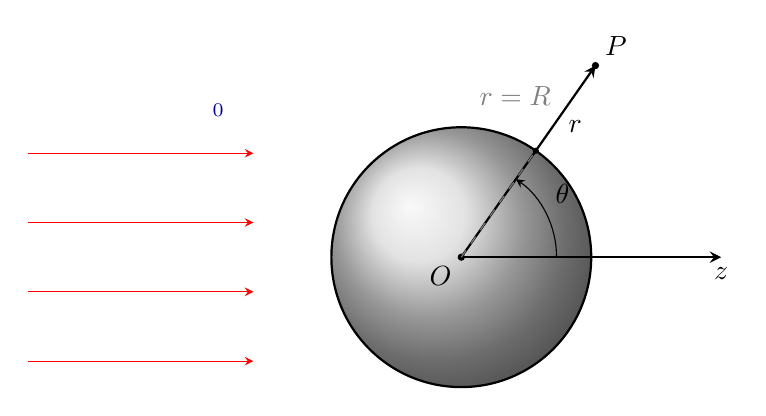
\begin{tikzpicture}[scale=1.1,>=stealth]

    % ---- куля ----
    \shade[ball color=gray!30] (0,0) circle (1.5);
    \draw[thick] (0,0) circle (1.5);

    % ---- центр і початок координат ----
    \fill (0,0) circle (1.2pt);
    \node[below left] at (0,0) {$O$};

    % ---- полярна вісь уздовж E_0 ----
    \draw[->,thick] (0,0) -- (3,0)
        node[below] {$z$};

    % ---- радіус-вектор r і кут theta ----
    \coordinate (P) at (55:2.7);
    \draw[->,thick] (0,0) -- (P)
        node[anchor=north west, pos=0.75, inner sep=2pt] {$\vect{r}$};
    \fill (P) circle (1.2pt);
    \node[above right] at (P) {$P$};

    % ---- кут theta ----
    \draw[->] (1.1,0) arc (0:55:1.1) node[pos=0.5, anchor=south west] {$\theta$};

    % ---- проекція на поверхню кулі ----
    \draw[dashed,gray] (0,0) -- (55:1.5);
    \fill (55:1.5) circle (1pt);
    \node[gray,above left] at (55:2) {$r=R$};

    % ---- зовнішнє поле (кілька стрілок) ----
    \foreach \y in {-1.2, -0.4, 0.4, 1.2} {
        \draw[->,red]
            (-5,\y) -- (-2.4,\y);
    }
    \node[blue!60!black] at (-2.8,1.7) {$\Efield_0$};

\end{tikzpicture}
\caption{Металева куля радіуса $R$ в однорідному зовнішньому полі
$\Efield_0$. Початок координат $O$ суміщено з центром кулі, полярну
вісь напрямлено вздовж $\Efield_0$. Положення точки $P$ задається
радіус-вектором $\vect{r}$ та кутом $\theta$ між $\vect{r}$ і
полярною віссю.}
\label{fig:sphere_in_field}
\end{figure}

\subsection*{Граничні умови на поле}

На поверхні металу $r = R$ мають виконуватися дві умови для поля.

\emph{Перша: тангенціальна складова неперервна.} Це загальна умова
для будь-якої межі поділу, і вона випливає з $\oint \Efield\cdot d\vect{l} = 0$:
\begin{equation*}
    E_{\tau}(R+0) = E_{\tau}(R-0) .
\end{equation*}
Оскільки всередині поля немає, $E_{\tau}(R-0) = 0$, а отже,
\begin{equation*}
    E_{\tau}(R+0) = 0 .
\end{equation*}
Це означає, що зовні поле підходить до поверхні кулі строго
перпендикулярно до неї.

\emph{Друга: стрибок нормальної складової.} Він визначається
поверхневим зарядом і випливає з теореми Гаусса:
\begin{equation*}
    E_{r}(R+0) - E_{r}(R-0) = \frac{\sigma}{\varepsilon_0}.
\end{equation*}
Оскільки $E_r(R-0) = 0$, маємо
\begin{equation*}
    \sigma = \varepsilon_0 E_r(R+0) .
\end{equation*}

Отже, вся задача зводиться до одного: знайти поле зовні кулі, яке
задовольняє дві умови --- воно перпендикулярне до поверхні та має
задану нормальну складову, яка й дає поверхневий заряд.

\subsection*{Поле зовні кулі}

Зовні кулі поле складається із зовнішнього однорідного поля
$\Efield_0$ та поля наведених зарядів на поверхні. Наведений заряд
в цілому нейтральний, тому його поле на великих відстанях
зменшується як поле диполя. Тому природно записати
\begin{equation*}
    \Efield(r,\theta) = \Efield_0 + \Efield_{\text{дип}},
\end{equation*}
де $\Efield_{\text{дип}}$ --- поле точкового диполя, орієнтованого
вздовж $\Efield_0$, з невідомим поки що моментом $\vect{p}$.

У сферичних координатах зручно працювати з компонентами. Для
однорідного поля, напрямленого вздовж осі $z$,
\begin{equation*}
    E_{0,r} = \Efield_0\cos\theta, \qquad
    E_{0,\theta} = -\Efield_0\sin\theta .
\end{equation*}
Для диполя з моментом $\vect{p} = p\,\hat{\vect z}$:
\begin{equation*}
    E_{\text{дип},r} = \frac{2p\cos\theta}{r^3}, \qquad
    E_{\text{дип},\theta} = \frac{p\sin\theta}{r^3} .
\end{equation*}

Повне поле зовні:
\begin{equation*}
    E_r = \Efield_0\cos\theta + \frac{2p\cos\theta}{r^3}, \qquad
    E_\theta = -\Efield_0\sin\theta + \frac{p\sin\theta}{r^3} .
\end{equation*}

\subsection*{Застосування граничних умов}

Підставляємо $r = R$.

З умови $E_\theta(R) = 0$:
\begin{equation*}
    -\Efield_0\sin\theta + \frac{p\sin\theta}{R^3} = 0
    \quad\Longrightarrow\quad
    p = \Efield_0 R^3 .
\end{equation*}

З умови $\sigma = \varepsilon_0 E_r(R)$:
\begin{equation*}
    \sigma(\theta) = \varepsilon_0
    \left( \Efield_0\cos\theta + \frac{2p\cos\theta}{R^3} \right)
    = \varepsilon_0 \left( \Efield_0\cos\theta
    + 2\Efield_0\cos\theta \right)
    = 3\varepsilon_0 \Efield_0\cos\theta .
\end{equation*}

Отже, обидві граничні умови дали повний розв'язок: і наведений
дипольний момент, і розподіл поверхневого заряду.

\subsection*{Остаточні результати}

Дипольний момент кулі:
\begin{equation*}
    \vect{p} = R^3\Efield_0 .
\end{equation*}

Поле зовні та всередині кулі:
\begin{equation*}
    \Efield =
    \begin{cases}
        0, & r \le R, \\[6pt]
        \Efield_0 - \dfrac{\vect{p}}{r^3}
        + \dfrac{3\left(\vect{p}\cdot\vect{r}\right)\vect{r}}{r^5},
        & r > R .
    \end{cases}
\end{equation*}

Заряди на поверхні:
\begin{equation*}
    \sigma = 3\varepsilon_0 \Efield_0\cos\theta
    = \frac{3}{4\pi}\,\frac{\Efield_0\cdot\vect{r}}{R}
    \quad\text{(у гауссовій системі)} .
\end{equation*}

Потенціал кулі (для повноти, його легко відновити інтегруванням поля):
\begin{equation*}
    \phi =
    \begin{cases}
        0, & r \le R, \\[4pt]
        -\left(\Efield_0\cdot\vect{r}\right)
        + \dfrac{\vect{p}\cdot\vect{r}}{r^3}, & r > R .
    \end{cases}
\end{equation*}

\begin{figure}[h!]
    \centering
    \localinput{EfieldMetall.tikz}
    \caption{Конфігурація поля навколо металевої кулі, вміщеної
    в однорідне електричне поле.\label{tikz:EfieldMetall}}
\end{figure}

%% --------------------------------------------------------
\section{Сили, що діють на поверхню провідника в полі}
%% --------------------------------------------------------


На малий елемент $dS$ поверхні провідника діє сила:
\begin{equation*}
	dF = dq E_0 = \sigma dS \cdot  E_0,
\end{equation*}
з боку \emphx{поля $E_0$ інших зарядів} у місці
знаходження заряду $dq = \sigma dS$. Але прилад може виміряти \emphx{сумарне поле
	$E$}, тобто поле  \emphx{інших зарядів $E_0$} плюс \emphx{власне поле
	$E_{\sigma}$}, і  розрізнити їх не може!

\begin{SCfigure}[1.5][h!]%{0.34\linewidth}
    \centering
	\localinput{Fmetall.tikz}
    \caption{До виведення сили, що діє на поверхню провідника}
\end{SCfigure}

Задача полягає в тому, щоб виразити силу саме через сумарне поле.

Оскільки поле всередині провідника $E = 0$, то власне поле за модулем має дорівнювати
полю <<чужих>> зарядів:
\begin{equation*}
	E_0 = E_{\sigma},
\end{equation*}
це означає, що \emphx{густина заряду підлаштовується під зовнішнє поле}!


Гранична умова дає поле у вакуумі:
\begin{equation*}
	E = E_0 + E_{\sigma} = 2 E_0 = 4\pi\sigma.
\end{equation*}


Сила, що діє на одиницю поверхні провідника
\begin{equation*}
	\frac{dF}{dS} = f = \frac12 \sigma E = \frac{E^2}{8\pi}.
\end{equation*}



%=========================================================
\begin{problem}%
    Знайдіть силу взаємодії двох заряджених металевих пластин, що знаходяться на малій відстані
    одна від одної. Густина заряду кожної з пластин $\sigma$. Площа пластин $S$.

    Якщо пластини мають форму дисків радіуса $R$, чому буде дорівнювати сила взаємодії між ними на
    відстані $\ell \gg R$?
\end{problem}

%=========================================================
\begin{problem}%
    Металева сфера радіуса $R$ складена з двох півсфер. Визначити силу $F$, з якою відштовхуються
    ці півсфери, якщо повний заряд сфери дорівнює~$Q$.

    Відповідь: $F= \frac{Q^2}{8R^2}$.
\end{problem}